\documentclass[12pt,a4paper]{jreport}
\usepackage{KIT-j-master}
\usepackage{latexsym}
\usepackage{amsmath}
\usepackage{amssymb}
\usepackage{comment}
%\usepackage{graphicx}
%\usepackage{subeqn}
%\usepackage{eqnarray}
\usepackage{newtheorem_thesis}
\usepackage[dvipdfmx]{color}
\usepackage[dvipdfmx]{graphicx}
\usepackage{subfigure}
\usepackage{slashbox}
\usepackage{here}
\usepackage{cite}

%%%%%%%%%%%%%%%%%%%%%%%%%%%%%%%%%%%%%%%%%%%%%%%%%%%%%%%%%%%%%%%%%%%%%%%%%
%ソースコードを表示するための設定
%(テンプレートには無い設定・listings & jlistingをインストールすること)
%%%%%%%%%%%%%%%%%%%%%%%%%%%%%%%%%%%%%%%%%%%%%%%%%%%%%%%%%%%%%%%%%%%%%%%%%
\usepackage{ascmac}
\usepackage{here}
\usepackage{txfonts}
\usepackage{listings,jlisting}
\usepackage{bm}
\usepackage{lscape}

\lstdefinestyle{customC++}{
	language={C++},% 使用する言語
	tabsize=2,%
	basicstyle=\footnotesize,%
	commentstyle=\textit,%
	classoffset=1,%
	keywordstyle=\bfseries,%
	frame=tRBl,framesep=5pt,%
	showstringspaces=false,%
	numbers=left,stepnumber=1,numberstyle=\footnotesize,%
	breaklines=true,%        折り返しの設定
	breakatwhitespace=true,% 折り返しの設定
	lineskip=-0.3ex%  
}

\lstdefinestyle{customhtml}{
	language={html},% 使用する言語
	tabsize=2,%
	basicstyle=\footnotesize,%
	commentstyle=\textit,%
	classoffset=1,%
	keywordstyle=\bfseries,%
	frame=tRBl,framesep=5pt,%
	showstringspaces=false,%
	numbers=left,stepnumber=1,numberstyle=\footnotesize,%
	breaklines=true,%        折り返しの設定
	breakatwhitespace=true,% 折り返しの設定
	lineskip=-0.3ex%  
}

\lstdefinestyle{custompy}{
	language={python},% 使用する言語
  	basicstyle=\ttfamily\scriptsize,
 	commentstyle={\itshape \color[cmyk]{1,0.4,1,0}},
	classoffset=1,
	keywordstyle={\bfseries \color[cmyk]{0,1,0,0}},
	stringstyle={\ttfamily \color[rgb]{0,0,1}},
	frame=tRBl,
	framesep=5pt,
	showstringspaces=false,
	numbers=left,
	stepnumber=1,
	numberstyle=\tiny,
	tabsize=2,
}
\lstset{escapechar=@,style=customC++}

%\renewcommand{\lstlistingname}{リスト}
%\lstset{language=C++,%
%tabsize=2,%
%basicstyle=\footnotesize,%
%commentstyle=\textit,%
%classoffset=1,%
%keywordstyle=\bfseries,%
%frame=tRBl,framesep=5pt,%
%showstringspaces=false,%
%numbers=left,stepnumber=1,numberstyle=\footnotesize,%
%breaklines=true,%        折り返しの設定
%breakatwhitespace=true,% 折り返しの設定
%lineskip=-0.3ex%         行間をつめる設定
%}

\title{2D-LiDARとYOLOv8を用いた人追従システムの開発}
\author{金澤 祐典}
\eauthor{KANAZAWA Yusuke}
\school{金沢工業大学}
\major{工学部}
\course{ロボティクス学科}
\adviser{出村 公成}
\date{令和5年度\\2024年1月12日}

\begin{document}
\maketitle

%\pagestyle{headings}
\pagenumbering{roman}
\tableofcontents
\listoffigures
\listoftables
\newpage
\pagenumbering{arabic}
\setcounter{page}{1}

%%%%%%%%%%%%%%%%%%%%%%%%%%%%%%%%%%%%%%%%%%%%%%%%%%%%%%%%%%%%%%%%%%%%%%%%%
\chapter{序 論}
\section{はじめに}
近年の日本において、少子高齢社会による人手不足が課題となっている。2023年の65歳以上の
人口は3623万人であり、総人口に占める65歳以上の割合(以下、高齢化率)は29.1[\%]と過去最高である\cite{統計からみた我が国の高齢者}。
また、2070年での高齢化率は38.7[\%]に達し、2.6人に1人が65歳以上であると推計されている\cite{高齢化の現状と将来像}。
加速する少子高齢化により、就業者不足の問題が深刻化しており、解決策の1つとしてロボットによる
作業の自動化やサポートの導入が増えている。建設業では、2D-LiDARを用いた自動追従台車である
「かもーん」が建設現場で導入されており、運用実績を上げ続けている\cite{近年の建設工事用ロボット開発について}。
また、製造業では2D-LiDARを用いた協働運搬ロボットである「サウザー」が実用化されており、
「自動追従走行機能」によって運搬業務をサウザーで行うことができ、製造業界だけでなく空港や市役所
などの公共環境における導入例があり、世界各地で約400台の販売実績がある\cite{既存AGVを超える特長を持った協働運搬ロボット「サウザー」}。
以上のことから、2D-LiDARを用いた人追従ロボットへの需要と期待は増加し続けていることがわかる。\\ \indent
2D-LiDARを用いた人追従ロボットに関する手法には、深層学習を用いる手法
\cite{深層学習を用いた人追従機能の開発}
\cite{People Detection and Tracking Using LIDAR Sensors}
\cite{Temporal convolutional networks for multi-person activity recognition using a 2D LIDAR}
\cite{Tracking People in a Mobile Robot From 2D LIDAR Scans Using Full Convolutional Neural Networks for Security in Cluttered Environments}
、背景減算によって人の両脚部分を検出する手法
\cite{Tracking People Using Ankle-Level 2D LiDAR for Gait Analysis}
、AOAタグを2D-LiDARと組み合わせる手法
\cite{A Robust Autonomous Following Method for Mobile Robots in Dynamic Environments}
などがある。これらの手法では、主に距離データをもとに人の両脚部分を検出するが、
雑多な環境下では追従が不安定になる可能性があり、また実験環境に椅子や机などのオブジェクトが
なく、広域な経路での実験により人追従を評価している。2D-LiDARから提供される距離データでは、椅子や机などの
脚部分は人の両脚部分と類似しているため、誤検出により本来の追従対象ではないものに
追従してしまうという課題がある。\\ \indent
本プロジェクトでは、屋内環境による雑多な環境下での人追従システムの開発を目的とし、
2D-LiDARとYOLOv8を用いることで人の両脚部分を検出し、追従目標の特定処理を加えることで、
雑多な環境下での人追従が可能なシステムを開発する。

\section{論文構成}
本レポートの構成について述べる。第2章では、これまでの2D-LiDARを用いた人追従に関連する
従来研究について述べる。第3章では、本プロジェクトでの提案手法を述べる。
第4章では、提案手法による人追従能力の検証結果について述べる。
第5章では本プロジェクトをまとめ、結論及び今後の課題について述べる。
%%%%%%%%%%%%%%%%%%%%%%%%%%%%%%%%%%%%%%%%%%%%%%%%%%%%%%%%%%%%%%%%%%%%%%%%%
\chapter{従来研究}
\section{従来研究}
従来研究では、あらかじめ人のいない状態の空間において、2D-LiDARの値から、深層学習を用いた
人検出の手法がある。この手法では、雑多な環境における人の検出が不安定である。

\subsection{図の貼り方}

\begin{figure*}[b]
\begin{center}
\includegraphics[height=50mm,clip]{figure/collect_dataset_overview.eps}
\caption{Automatic annotation overview using the Fluoresent AR Marker}
\label{Automatic annotation overview using a Fluoresent AR marker}
\end{center}
\end{figure*}

\begin{figure*}[t]
\begin{center}
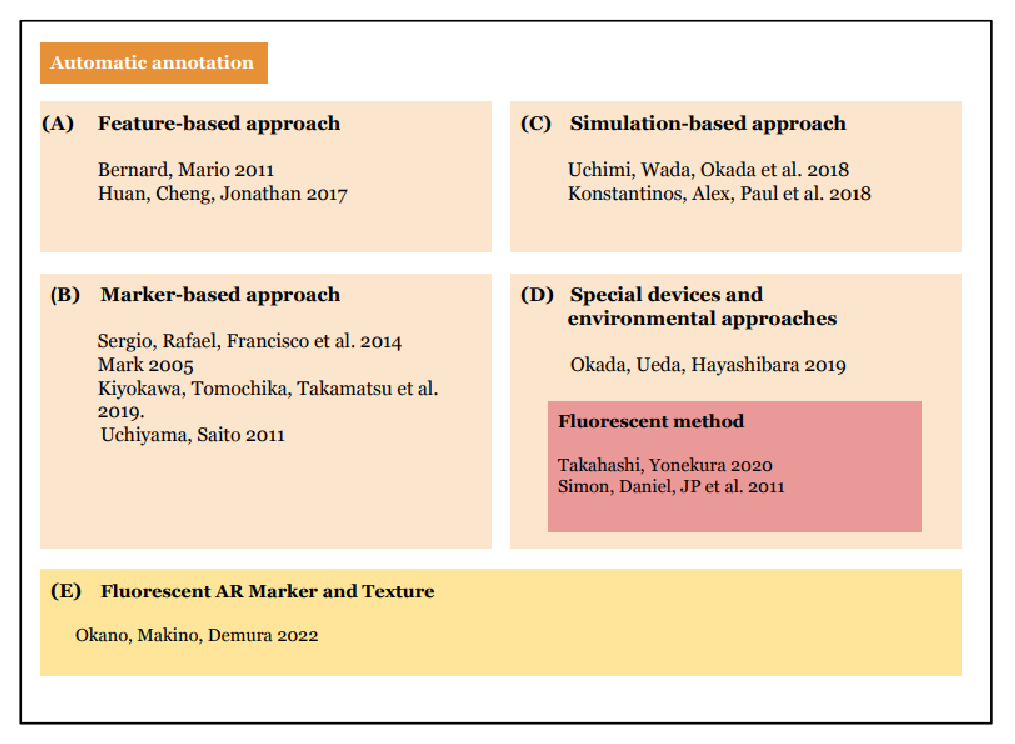
\includegraphics[width=160mm,clip]{figure/related_overview.eps}
\caption{Automatic annotation overview}
\label{Automatic annotation overview}
\end{center}
\end{figure*}

Fig. \ref{Automatic annotation overview}とFig. \ref{Automatic annotation overview using a Fluoresent AR marker}見てね!

\subsection{表の貼り方}
Table\ref{Hardware}を見てね!

\begin{table}[tb]
  \begin{center}
    \caption{{Equipment}\label{Hardware}}
    \scalebox{0.7}[0.9]{
      \begin{tabular}{|c|r|} \hline
        Microcomputer & Arduino Uno \\ \hline
        Motor & Dynamixel XM430-W350-R \\ \hline
        Communication converter & ROBOTIS, U2D2 SMPS2 \\ \hline
        Solid State Relays & Solid State Relays Kit Type 20A \\ \hline
        Visible light & Fluorescent LED light 40W \\ \hline
        UV light & TOSHIBA black light FL4BLB/N \\ \hline
        Camera & Realsense D435 \\ \hline
      \end{tabular}
    }
  \end{center}
\end{table}

\subsection{参考文献の引き方}
\cite{1}と\cite{2}を参考にする
%%%%%%%%%%%%%%%%%%%%%%%%%%%%%%%%%%%%%%%%%%%%%%%%%%%%%%%%%%%%%%%%%%%%%%%%%
\chapter{提案手法}
\section{概要}
本プロジェクトでは、雑多な環境下で人追従でき、ロボットの最大直進速度で追従するため、
2D-LiDARの距離データとリアルタイム物体検出アルゴリズムであるYOLOv8を用いた人追従システムを開発する。
本プロジェクトで提案する人追従システムは、追従対象者のみがいる雑多な環境を想定している。
雑多な環境では、人の脚部と形状が類似している椅子やポールなどの物体をランダムに多数
設置している。2D-LiDARから提供される距離データを俯瞰画像に変換し、
学習したYOLOv8と俯瞰画像を用いて追従対象者の検出をする。追従対象者の検出のみでは、
周囲の物体を両脚部と誤検出する可能性があるため、追従目標の特定処理をシステムに組み込む
ことで、正確に追従対象者を追従することを実現する。

\section{要求仕様}
本プロジェクトでは、雑多な環境下で人追従でき、ロボットの最大直進速度で追従できる人追従システムの
開発を目的としているため、以下の構成で要求仕様を設定する。
使用するロボットは、2023年に開催されたRoboCup 2023で開発したロボットである
Happy Eduを使用する。Happy Eduのロボット台車は、ROBOTIS社のTurtleBot3 Big Wheelであり、
ロボット台車の前方に2D-LiDARを搭載している。
2D-LiDARは、北陽電機株式会社のUTM30-LXを使用しており、ロボットに搭載するPCは、
NVIDIA GeForce RTX 4070 8GB を搭載しているノートPCを選定した。\\ \indent
以上の構成で以下の要求仕様を設定する。\\

\begin{enumerate}
\item 2D-LiDARのデータで人追従ができる。
\item 雑多な状態の空間でも人追従ができる。
\item 0.5[m/s]以下の歩行速度で追従する。
\end{enumerate}

\section{システム構成}
本プロジェクトでは、Fig. \ref{System configuration chart}のような人追従システムを提案する。
2D-LiDARから提供される距離データを俯瞰画像に変換し、YOLOv8のリアルタイム物体検出モデルにより
人の両脚部分を検出する。YOLOv8による人の両脚部分の検出は、別の物体を誤検出することがあるため、
追従目標の特定処理を実装している。追従対象の特定後、ロボットが追従すべき目標座標を生成し、
ロボットから目標座標までの距離と角度の偏差を収束させるため、PID制御によりロボット台車を制御する。

\begin{figure*}[h]
    \begin{center}
    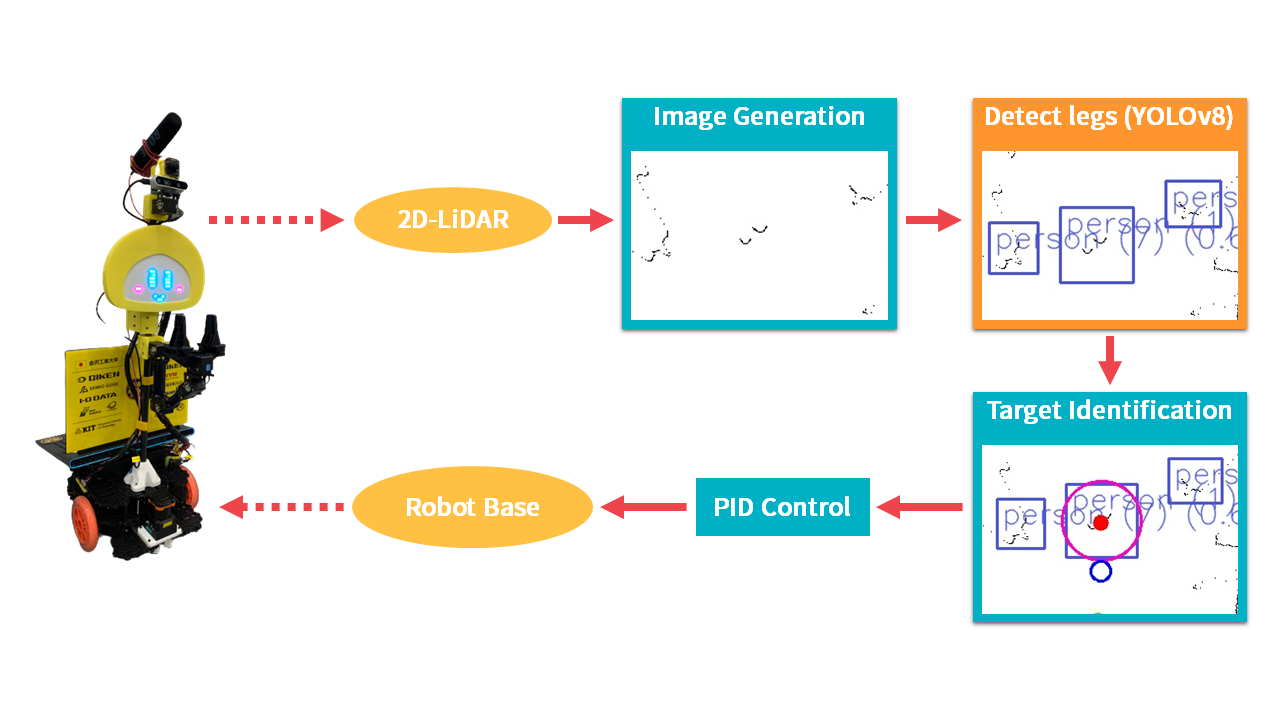
\includegraphics[height=100mm,clip]{figure/System-configration-chart.png}
    \caption{System configuration chart}
    \label{System configuration chart}
    \end{center}
\end{figure*}

\section{ソフトウェア構成}
ロボット用ノートPC内のソフトウェア構成をFig. \ref{Software configuration diagram}に示す。
ロボット用ノートPCのオペレーティングシステムにはUbuntu 22.04 LTSを使用し、ミドルウェアには
Robot Operationg System 2 (以下、ROS2)を用いている。ロボットのソフトウェア開発には、
主にPython言語を使用し、YOLOv8のROS2パッケージにはyolov8\_rosパッケージを用いている。
今回開発した人追従システムは、ROS2パッケージになっており、Fig. \ref{Software configuration diagram}
のfollow\_me Package上の構成となっている。follow\_me Package上には、laser\_to\_image Node、
person\_detector Node、base\_controller Nodeがあり、ソースコードの可読性を上げるため
このような構成にしている。また、ノード (Node) とは、ROS2でソフトウェア開発する上での最小単位である。\\ \indent
各ノードの処理内容は以下の通りである。

\begin{itemize}
    \item YOLOv8 Nodes: 俯瞰画像から人の両脚部分を検出する。
    \item laser\_to\_image Node: 2D-LiDARの距離データを俯瞰画像に変換する。
    \item person\_detector Node: 推論結果をもとに、追従目標を特定し目標座標を生成する。
    \item base\_controller Node: 目標座標までの距離と角度の偏差をPID制御により収束させる。
\end{itemize}

\begin{figure*}[h]
    \begin{center}
    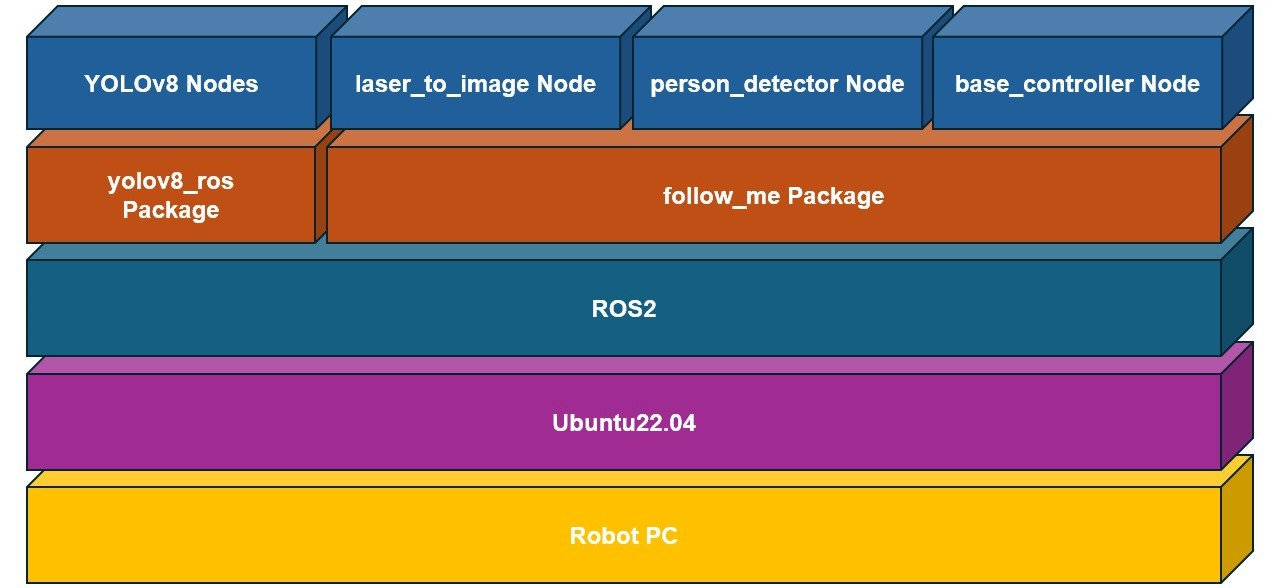
\includegraphics[height=80mm,clip]{figure/Software.jpg}
    \caption{Software configuration diagram}
    \label{Software configuration diagram}
    \end{center}
\end{figure*}

\section{データセットの作成}
データセットを作成するため、2D-LiDARの距離データを収集する。
データ収集時の環境は、ロボットが静止した状態においてロボットの前方で2人の人が歩行する。
データ収集中の2人の歩行パターンを以下に示す。
方向については、ロボットからみた方向である。
\begin{itemize}
    \item 左から右方向に歩行する。
    \item 右から左方向に歩行する。
    \item 手前から奥方向に歩行する。
    \item 奥から手前方向に歩行する。
    \item 右手前から左奥方向に歩行する。
    \item 左奥から右手前方向に歩行する。
    \item 左手前から右奥方向に歩行する。
    \item 右奥から左手前方向に歩行する。
    \item 人同士が交差する。
\end{itemize}
また、歩行時の歩幅については以下に示す。
\begin{itemize}
    \item 普段通りの歩幅で歩行する。
    \item 大股(歩幅、足4つ分程度)で歩行する。
    \item 小股(歩幅、足2つ分程度)で歩行する。
\end{itemize}
以上を5分間でランダムに行い、2D-LiDARの距離データをトピック通信によってトピックとして配布し、
ROS2 Bagを用いて保存する。
トピック通信とは、ROS2における通信手法のことであり、トピック通信によって送受信されるデータがトピックである。
また、ROS2 Bagは、ROS2におけるトピックの保存機能である。\\ \indent
ROS2 Bagのデータから、2D-LiDARの距離データをFig. \ref{Example of an overhead view image}
のような俯瞰画像へ変換する。変換方法を以下に示す。
\begin{enumerate}
    \item 白画像を生成する。
    \item 2D-LiDARからの距離データと1ステップあたりの角度を取得する。
    \item 距離データと1ステップあたりの角度から、距離データを画像の左上端を原点としたXY座標に変換する。
    \item 変換したXY座標から、点を白画像に黒点でプロットする。
\end{enumerate}
以上の方法で、2D-LiDARの距離データから12032枚の画像データを生成した。\\ \indent
画像データからデータセットを作成する。
人の両脚部分をpersonクラスとしてアノテーションを行った。アノテーションは、labelImgを用いて手動で行った。
labelImgとは、GUIでアノテーションが可能なアノテーションツールであり、ファイルの出力
形式としてYOLO形式がある。ファイル形式はYOLO形式で出力した。
また、データセットには、画像の回転処理、モザイク処理、2枚の
画像を合成し、新しく1枚の画像を生成する Mix Up 処理をすることでデータ拡張を行い、
計21061枚のデータセットを作成した。
Fig. \ref{Example data sets}にデータセットの例を示す。

\begin{figure*}[h]
    \begin{center}
    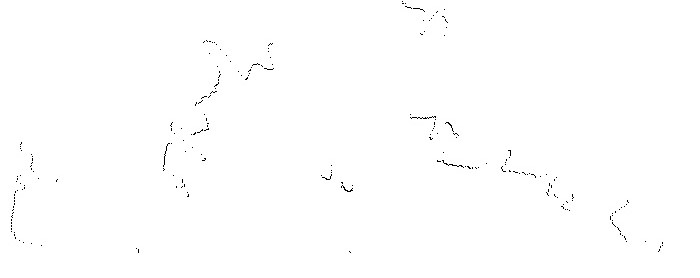
\includegraphics[height=50mm,clip]{figure/laser_img_232.jpg}
    \caption{Example of an overhead view image}
    \label{Example of an overhead view image}
    \end{center}
\end{figure*}

\begin{figure*}[h]
    \begin{center}
    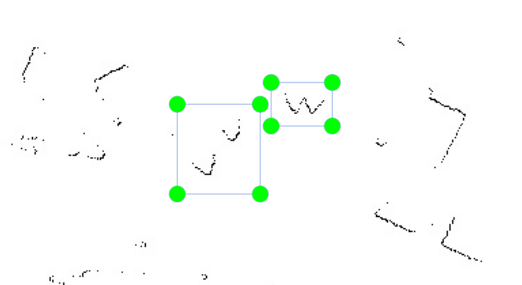
\includegraphics[height=60mm,clip]{figure/Example-data-sets.png}
    \caption{Example data sets}
    \label{Example data sets}
    \end{center}
\end{figure*}

\section{YOLOv8による学習}
作成したデータセットとYOLOv8を用いて人の両脚検出器を作成する。
学習には、リアルタイム物体検出アルゴリズムであるYOLO (You Only Look Once)を使用し、
学習モデルの初期重みは、ロボットに搭載するノートPCの性能が高いため、最もパラメータ数
の多いYOLOv8xを選定した。学習するPCは、NVIDIA GeForce RTX 4090 16GBを搭載している
PCを使用し、バッチサイズは12、エポック数は500で学習を行った。過学習を防ぐため、
過学習が発生する直前または発生したらすぐに学習を終了させる処理を100エポック以降で設定した。
学習結果は、Fig. \ref{Training results}とFig. \ref{Example of inference results with YOLOv8 using learned weights}
のようになっており、推論結果が90[\%]を超えていることが分かる。

\begin{figure*}[h]
    \begin{center}
    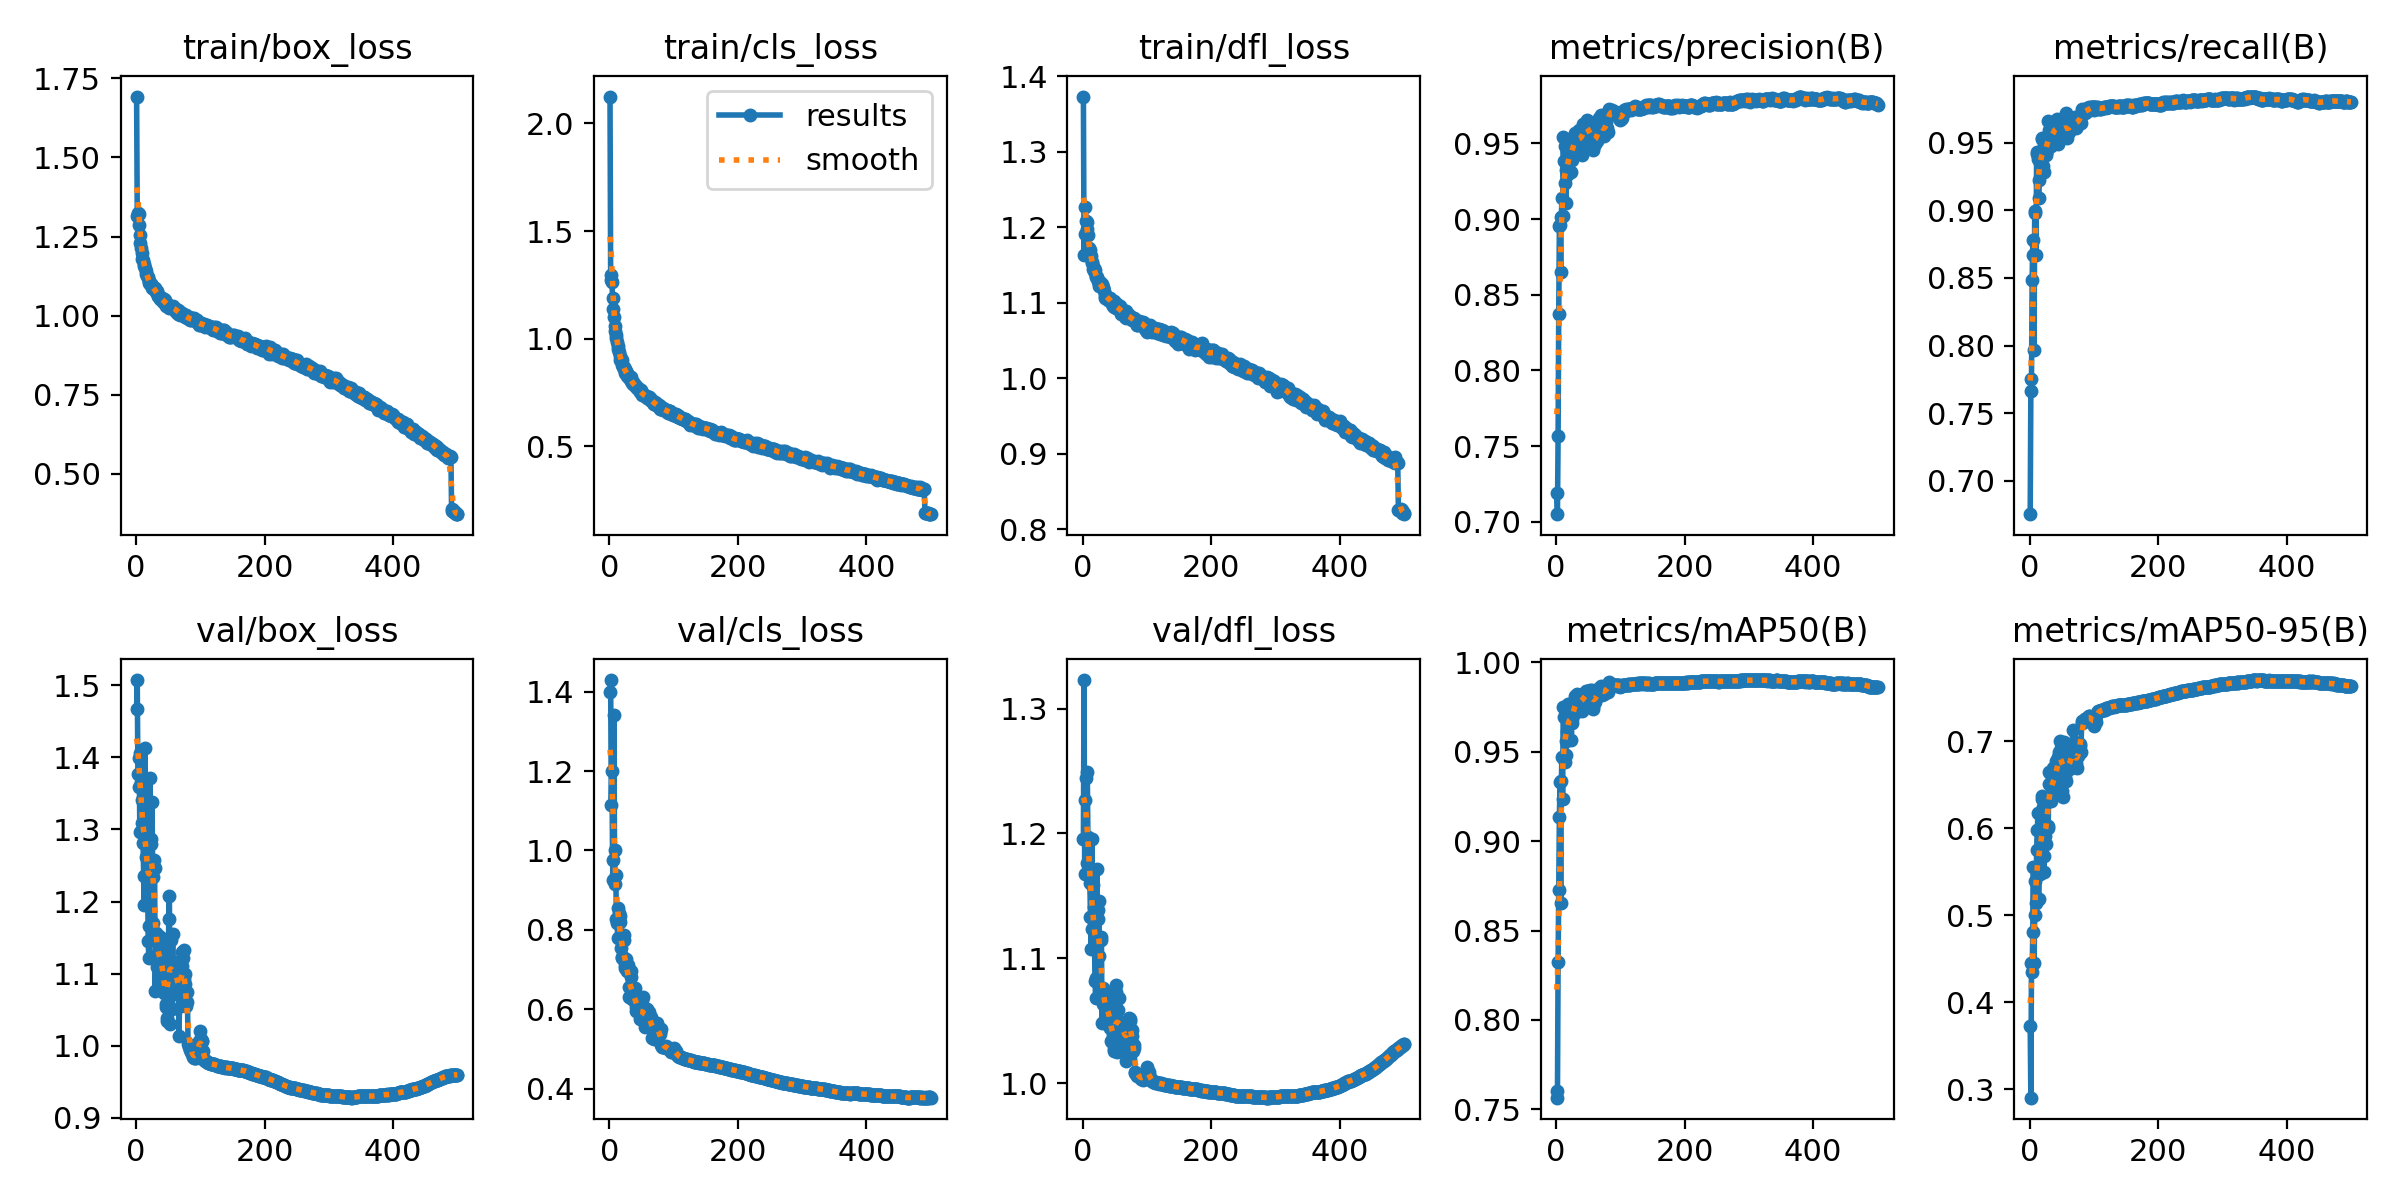
\includegraphics[height=70mm,clip]{figure/yolov8-train-results.png}
    \caption{Training results}
    \label{Training results}
    \end{center}
\end{figure*}

\begin{figure*}[h]
    \begin{center}
    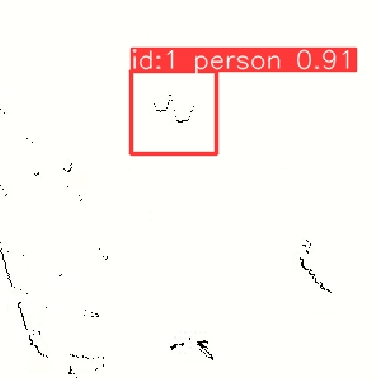
\includegraphics[height=60mm,clip]{figure/yolov8_laser_img.png}
    \caption{Example of inference results with YOLOv8 using learned weights}
    \label{Example of inference results with YOLOv8 using learned weights}
    \end{center}
\end{figure*}

\section{追従目標の特定}
YOLOv8による推論結果を用いて追従目標の特定をする。
前節で作成した両脚検出器では、Fig. \ref{yolo image}のように複数検出される場合があり、
追従目標を特定する必要がある。
YOLOv8には、Byte Trackなどの追跡アルゴリズムが標準機能で搭載されており、検出した物体
にIDを付与することができる。しかし、1度検出を外れ、再度同じ物体が検出されてもIDが変わって
しまうという問題がある。そこで、動的検出範囲を実装することで追従目標を特定する。\\ \indent
本プロジェクトで実装した追従目標の特定方法をFig. \ref{Target identification methods}
に示す。1フレーム前における追従目標のバウンディングボックスを中心とした、半径0.5[m]の
円型範囲を現在のフレームに設定し、範囲内にバウンディングボックスの中心があればそれを
追従対象とする。

\begin{figure*}[h]
    \begin{center}
    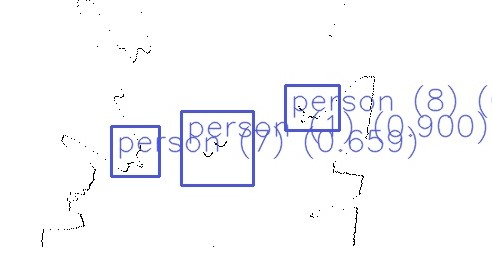
\includegraphics[height=50mm,clip]{figure/yolo_image.jpg}
    \caption{Multiple leg sections detected on both legs}
    \label{yolo image}
    \end{center}
\end{figure*}

\begin{figure*}[h]
    \begin{center}
    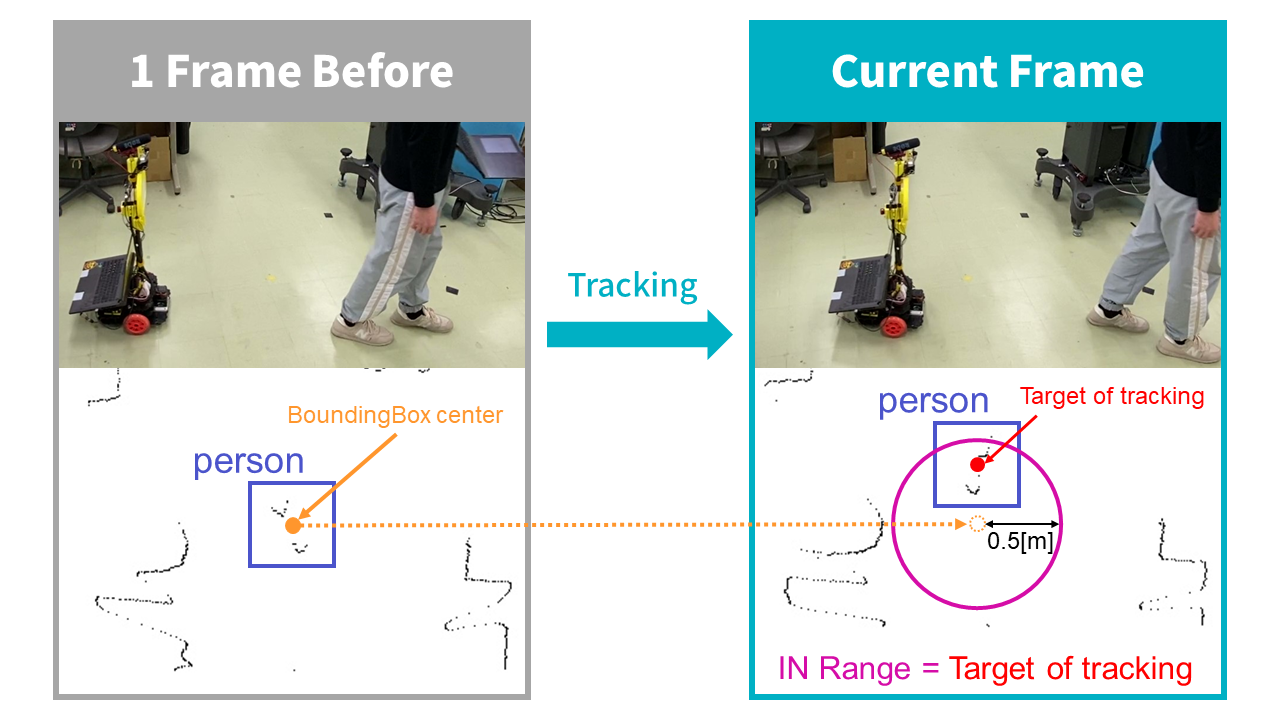
\includegraphics[height=70mm,clip]{figure/Target-identification-methods.png}
    \caption{Target identification methods}
    \label{Target identification methods}
    \end{center}
\end{figure*}

\section{ロボット台車の制御}
追従目標の特定により、追従目標のバウンディングボックスの中心から後方に定数で目標座標を生成
し、ロボットから目標座標までの距離と角度の偏差を収束させるためPID制御を実装した。 \\ \indent
時刻$t$での、ロボットの座標から目標座標までの角度の偏差を$\theta(t)$とし、ロボット台車の
エンコーダから取得できる旋回速度を$\omega(t)$とする。また、追従目標への角度の偏差が3.0[deg]
未満である場合に積分制御を開始する時刻を$t_1$としたとき、
ロボット台車の旋回速度の制御量$u_{angle1}(t)$は以下のようになる。
\begin{equation}
\label{angularPID}
u_{angle1}(t) = K_{AP} \cdot \theta(t) + K_{AI} \cdot \int_{t_1}^{t-t_1} \theta(\tau) d\tau + K_{AD} \cdot \left\{ \frac{d}{dt} \theta(t) - \omega(t) \right\}
\end{equation}
また、追従目標への角度の偏差が3.0[deg]以上である場合はPD制御に切り替える。
PD制御時の制御量$u_{angle2}(t)$は以下のようになる。
\begin{equation}
\label{angularPD}
u_{angle2}(t) = K_{AP} \cdot \theta(t) + K_{AD} \cdot \left\{ \frac{d}{dt} \theta(t) - \omega(t) \right\}
\end{equation}
$K_{AP}$、$K_{AI}$、$K_{AD}$はPIDゲインであり、$K_{AP}$は0.005、$K_{AI}$は0.0002、
$K_{AD}$は0.0009で設定している。PIDゲインの設定値は、Pゲイン、Dゲイン、Iゲインの順に設定した。
Pゲインでは、ロボット台車が左右に振動する1つ前の値を設定している。
Dゲインでは、P制御による小さい振動が発生しなくなる値を設定している。
Iゲインでは、ロボット台車の並進制御をしない状態において、
追従目標への角度の偏差の定常偏差が0.1[deg]未満になる値を設定している。
(\ref{angularPID})式の第1項は、ロボットの座標から目標座標
までの角度の偏差を比例制御している。第2項は、ロボットが追従対象者の方向を定常偏差なく向く
ため、目標座標までの角度の偏差を積分制御している。第3項では、実機での制御を考慮し、
過多な制御量を微分制御により調整している。また、(\ref{angularPD})式のようにPD制御に切り替えるのは、
角度の偏差が大きくなった場合に、積分値が時間経過に伴い過多になりすぎることで、
ロボットが左右に振動してしまうからである。\\ \indent
また、追従目標への距離の偏差を$l(t)$としたとき、ロボット台車の直進速度の制御量$u_{linear}(t)$
は以下のようになる。
\begin{equation}
\label{linearPID}
u_{linear}(t) = K_{LP} \cdot l(t)
\end{equation}
$K_{LP}$はPゲインである。(\ref{linearPID})式は、追従目標への距離の偏差を比例制御しており、
$K_{LP}$は0.3で設定している。
Pゲインは、ロボット台車が前後方向に振動する1つ前の値を設定している。


%%%%%%%%%%%%%%%%%%%%%%%%%%%%%%%%%%%%%%%%%%%%%%%%%%%%%%%%%%%%%%%%%%%%%%%%%
\chapter{実験}
\section{実験方法}
実験では、要求仕様(2)を検証するため、雑多な環境を作成し追従実験をする。
雑多な環境では、Fig 5 (a)のような環境を想定し、人間は追従対象の1人のみとする。
実験する経路は、直線経路、曲線経路、直角経路をそれぞれ10回実験する。
また、要求仕様(3)を検証するため、Fig 5 (b)のような10[m]での直線経路にて最大追従速度実験をする。
0.1[m/s]から、0.1ずつ速度を上昇させ、追従できなくなる速度の直前を最大追従速度とする。
要求仕様(2)、(3)が満たされたら、要求仕様(1)も満たされたものとする。

\section{実験結果}

%%%%%%%%%%%%%%%%%%%%%%%%%%%%%%%%%%%%%%%%%%%%%%%%%%%%%%%%%%%%%%%%%%%%%%%%%
\chapter{結 言}
\section{結言}

おわりおわりおわりおわりおわりおわりおわりおわりおわりおわりおわりおわりおわりおわりおわりおわりおわりおわりおわりおわりおわりおわりおわりおわりおわりおわりおわりおわりおわりおわりおわりおわりおわりおわりおわりおわりおわりおわりおわりおわりおわりおわりおわりおわりおわりおわりおわりおわりおわりおわりおわりおわりおわりおわりおわりおわりおわり
%%%%%%%%%%%%%%%%%%%%%%%%%%%%%%%%%%%%%%%%%%%%%%%%%%%%%%%%%%%%%%%%%%%%%%%%%
\chapter*{謝 辞}
%謝辞

 本研究を行うにあたり全体を通してご指導、ご教授、議論などのご助力をいただきました本学ロボティクス学科の出村公成教授に深く感謝いたします。

\begin{flushright}
令和4年2月
\end{flushright}

%%%%%%%%%%%%%%%%%%%%%%%%%%%%%%%%%%%%%%%%%%%%%%%%%%%%%%%%%%%%%%%%%%%%%%%%%
\begin{thebibliography}{99}

    \bibitem{1}%1
    宮口幹太, “近年の建設工事用ロボット開発について” 計測と制御 第61巻 第9号, p. 641-644, 2022.
    
    \bibitem{2}%2
    L.~Yi, V.~G.~Kim, D.~Ceylan, I.~C.~Shen, M.~Yan, H.~Su, C.~Lu,
    Q.~Huang, A.~Sheffer, L.~Guibas, “A scalable active framework for region annotation in 3d shape collections,” ACM Transactions on Graphics, Vol. 35, No. 6, p. 1–31, 2016.

\end{thebibliography}
%%%%%%%%%%%%%%%%%%%%%%%%%%%%%%%%%%%%%%%%%%%%%%%%%%%%%%%%%%%%%%%%%%%%%%%%%

%%%%%%%%%%%%%%%%%%%%%%%%%%%%%%%%%%%%%%%%%%%%%%%%%%%%%%%%%%%%%%%%%%%%%%%%%
\chapter*{本研究に関する学術発表論文}
%%%%%%%%%%%%%%%%%%%%%%%%%%%%%%%%%%%%%%%%%%%%%%%%%%%%%%%%%%%%%%%%%%%%%%%%%
%本研究に関する学術発表論文

%%%%%%%%%%%%%%%%%%%%%%%%%%%%%%%%%%%%%%%%%%%%%%%%%%%%%%%%%%%%%%%%%%%%%%%%%
\end{document}
